\chapter{曲线运动}
\section{曲线运动}
\subsection{定义}
 物体运动时轨迹为曲线的运动叫做曲线运动.
\subsection{曲线运动的位移和速度}
\subsubsection{位移}
物体的位移是由初位置指向末位置的\CJKunderwave{有向}线段.当物体做曲线运动时,可建立平面直角坐标系,物体的位移可以用它在坐标轴方向的\CJKunderwave{投影}来表示.

\subsubsection{速度}

质点做曲线运动时,速度的方向是时刻\CJKunderwave{改变}的,质点在某一时刻(或者某一位置)速度的方向与这一时刻质点所在位置处曲线的\CJKunderwave{切线}的方向一致.

对于曲线运动的速度的描述,可以将速度分解为相互垂直的两个分速度,在分解时遵循\CJKunderwave{平行四边形定则}.如图 \ref{fig:parabola} 所示,借用平抛运动的运动轨迹图象来说明各物理量的意义.

\begin{figure}[H]
  \centering
  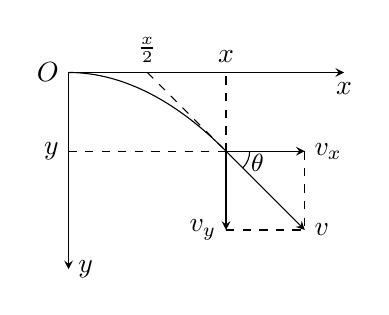
\begin{tikzpicture}
    \draw [->,>=stealth] (0,0) node [anchor= east] {$O$}--(3.5,0) node [anchor=north]{$x$};
    \draw [->,>=stealth] (0,0)--(0,-2.5) node [anchor=west]{$y$};
    \draw (0,0) parabola (2,-1);
    \draw [dashed] (1,0) node [anchor=south] {\small $\frac{x}{2}$} -- (2,-1);
    \draw [dashed] (2,-1) --(2,0) node [anchor=south] {$x$};
    \draw [dashed] (2,-1) -- (0,-1) node [anchor=east] {$y$};
    \draw [->,>=stealth] (2,-1) -- (3,-2) node [anchor=west] {$v$};
    \draw [->,>=stealth] (2,-1) -- (3,-1) node [anchor=west] {$v_x$};
    \draw [->,>=stealth] (2,-1) -- (2,-2) node [anchor=east] {$v_y$};
    \draw [dashed] (3,-1) -- (3,-2);
    \draw [dashed] (2,-2) -- (3,-2);
    \draw (2.2122,-1.2122) arc (315:360:0.3);
    \draw (2.4,-1.15) node {\small $\theta$};
  \end{tikzpicture}
  \caption{平抛运动}
  \label{fig:parabola}
\end{figure}


对两个分速度的定义分别是:
\begin{equation}
v_x =\frac{\Delta x}{\Delta t} ,v_y =\frac{\Delta y}{\Delta t}
\end{equation}
如果速度与$x$ 轴的夹角为$\theta$ , 则由平行四边形定则得:
\begin{equation}
v_x=v\cos\theta , v_y=v\sin\theta
\end{equation}

由分速度求合速度,则根据勾股定理得
\begin{gather}
  v=\sqrt{v_x^2+v_y^2}\\
  \tan\theta=\frac{v_y}{v_x}
\end{gather}

\subsection{曲线运动的性质及分类}

由于速度是矢量,物体做曲线运动时速度方向一定是发生变化的,所以曲线运动一定是\CJKunderwave{变速运动}.

如果物体做曲线运动时\CJKunderwave{加速度恒定},则叫做匀变速曲线运动.如果物体做曲线运动时\CJKunderwave{加速度是变化的},则叫做非匀变速曲线运动.

\subsection{物体做曲线运动的条件}

当合力的方向(或者加速度的方向)与速度方向\CJKunderwave{不在一条直线上时}物体将做曲线运动.这含有三个层次的内容:1.初速度不为零,2.合力不为零,3.合力的方向与速度方向不在同一直线上.

\subsection{曲线运动的轨迹特点}

做曲线运动的物体的轨迹与速度方向相切,并且向力的方向弯曲.也就是合力指向轨迹凹侧.

\subsection{例题分析}
\begin{selection}
  1.如<:
  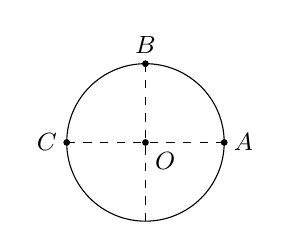
\begin{tikzpicture}
    \draw (0,0) circle [radius=1];
    \filldraw [black] (0,0) node [anchor=north west] {\small $O$} circle [radius=1pt];
    \filldraw [black] (1,0) node [anchor=west] {\small $A$} circle [radius=1pt];
    \filldraw [black] (-1,0) node [anchor=east] {\small $C$} circle [radius=1pt];
    \filldraw [black] (0,1) node [anchor=south] {\small $B$} circle [radius=1pt];
    \draw [dashed] (-1,0) -- (1,0);
    \draw [dashed] (0,-1) -- (0,1);
  \end{tikzpicture}
  :>所示,一个质点做圆周运动,A、B、C是其轨迹上的三点.下列说法正确的是
  A.质点可能做匀速运动
  B.质点一定做变速运动
  C.质点受到的合力可能等于零
  D.质点经过A、C两点时的速度相同

  a.B

  e.质点的轨迹是曲线,则速度一定发生变化,所以不可能匀速,一定是变速运动.物体做曲线运动的条件是合力与速度的方向不共线,则合力一定不为零,同时根据牛顿第一定律也可以得到合力为零则物体做匀速直线运动,所以A,C错误.同时,质点到达A点和C点时速度的方向一定相反,所以速度不相同.

2.如<:
\begin{tikzpicture}
  \draw (0,0) node [anchor=north] {\small $A$}  .. controls (0.3,0.6) .. (1,1) node [anchor=south east] {\small $B$};
  \draw [dashed] (1,1) -- (1.6,1.6) node [anchor=south west] {\small $b$};
  \draw [dashed] (1,1) .. controls (1.1,1.4) .. (0.8,1.8) node [anchor=west] {\small $c$};
  \draw [dashed] (1,1) .. controls (1.9,1.3) .. (2,0.5) node [anchor=west] {\small $a$};
\end{tikzpicture}
:>所示,物体在恒力F作用下沿曲线从点 $A$ 运动到点 $B$,这时突然使它所受的力反向,但大小不变,即由$F$ 变为 $-F$. 在此力的作用下,物体以后的运动情况,下列说法正确的是
A.物体可能沿曲线 $Ba$ 运动 
B.物体可能沿曲线 $Bb$ 运动
C.物体可能沿曲线 $Bc$ 运动
D. 物体可能沿原曲线 $BA$ 返回

a.C

e.物体从A到B运动,因为运动轨迹是在速度与力的夹角之中,所以物体所受的恒力方向是向下的.到达B点后,力的大小不变方向相反,变成向上.所以轨迹Bc就落在了力与速度的夹角内,则物体有可能沿Bc运动 ,则C正确.

\end{selection}
\newpage
\begin{calculate}
  1.质量为$m=2kg$ 的物体在光滑水平面上运动,其分速度 $v_x$ 和 $v_y$随时间变化的图线如<:
  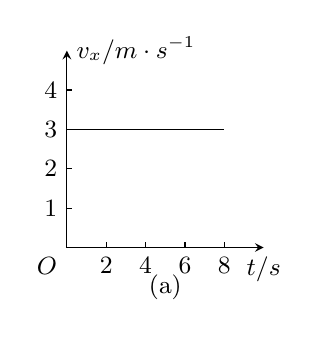
\begin{tikzpicture}
    \draw[->,>=stealth] (0,0) node [anchor=north east] {\small $O$} -- (2.5,0) node [anchor=north] {\small $t/s$};
    \draw (0.5,0) node [anchor=north] {\small 2}-- (0.5,2pt);
    \draw (1,0) node [anchor=north]{\small 4} -- (1,2pt);
    \draw (1.5,0) node [anchor=north]{\small 6} -- (1.5,2pt);
    \draw (2,0) node [anchor=north]{\small 8} --(2,2pt);
    \draw [->,>=stealth] (0,0) -- (0,2.5) node [anchor=west] {\small $v_x/m\cdot s^{-1}$};
    \draw (0,0.5) node  [anchor=east] {\small 1} -- (2pt,0.5);
    \draw (0,1) node  [anchor=east] {\small 2} -- (2pt,1);
    \draw (0,1.5) node  [anchor=east] {\small 3} -- (2pt,1.5);
    \draw (0,2) node  [anchor=east] {\small 4} -- (2pt,2);
    \draw (0,1.5) --(2,1.5);
    \draw (1.25,-0.5) node {\small (a)};
  \end{tikzpicture}
  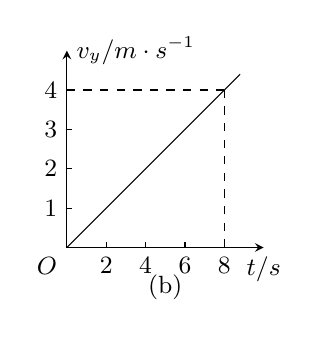
\begin{tikzpicture}
    \draw[->,>=stealth] (0,0) node [anchor=north east] {\small $O$} -- (2.5,0) node [anchor=north] {\small $t/s$};
    \draw (0.5,0) node [anchor=north] {\small 2}-- (0.5,2pt);
    \draw (1,0) node [anchor=north]{\small 4} -- (1,2pt);
    \draw (1.5,0) node [anchor=north]{\small 6} -- (1.5,2pt);
    \draw (2,0) node [anchor=north]{\small 8} --(2,2pt);
    \draw [->,>=stealth] (0,0) -- (0,2.5) node [anchor=west] {\small $v_y/m\cdot s^{-1}$};
    \draw (0,0.5) node  [anchor=east] {\small 1} -- (2pt,0.5);
    \draw (0,1) node  [anchor=east] {\small 2} -- (2pt,1);
    \draw (0,1.5) node  [anchor=east] {\small 3} -- (2pt,1.5);
    \draw (0,2) node  [anchor=east] {\small 4} -- (2pt,2);
    \draw (0,0) --(2.2,2.2);
    \draw [dashed] (2,0) -- (2,2);
    \draw [dashed] (0,2) -- (2,2);
    \draw (1.25,-0.5) node {\small (b)};
  \end{tikzpicture}
  :>所示,求:
  [1]物体所受的合力
  [2]物体的初速度
  [3] $t=8s$ 时物体的速度
  [4] $t=4s$ 内物体的位移

a.见解析

e.(1)由图(a)可得
$$a_x=\cfrac{\Delta v_x}{\Delta t}=0m/s^2$$
由图(b)可得
$$a_y=\cfrac{\Delta v_y}{\Delta t}=\cfrac{4-0}{8-0}m/s^2=0.5m/s^2$$
所以加速度大小为 $0.5m/s^2$ 方向沿$y$轴正方向.

ee.(2)$t=0s$时,$v_{x0}=3m/s$,$v_{y0}=0m/s$ ,所以物体的初速度为
$$v_0=3m/s$$
方向沿$x$轴正方向.

ee.(3)当$t=8s$时,$v_x=3m/s$,$v_y=4m/s$ ,所以物体的速度为
$$v=\sqrt{v_x^2+v_y^2}=5m/s$$
$$\tan \theta =\cfrac{v_y}{v_x}=\cfrac{4}{3}$$
所以得 $\theta = 53^\circ$ ,即速度大小为$5m/s$ 方向与$x$轴正方向所成角度为$53^\circ$

ee.由图象面积表示位移可得
$$x=v_x t = 12m$$
$$y=\cfrac{1}{2}a_yt^2=\cfrac{1}{2}\times 0.5 \times 4^2 m=4m$$
由位移的合成可得
$$l=\sqrt{x^2+y^2}=2\sqrt{10}m$$
位移与水平方向的夹角$\alpha$ 为
$$\tan \alpha =\cfrac{y}{x}=\cfrac{1}{3}$$


\end{calculate}

\section{平抛运动}

\subsection{定义}
平抛运动是一类最简单的曲线运动,当物体的初速度沿水平方向,且只受重力时,物体运动的轨迹为抛物线,所以这类运动叫做平抛运动.如果物体的初速度方向与水平方向有一定的夹角,则叫做抛体运动.所以总结物体做平抛运动的条件为:
\begin{enumerate}
  \item 初速度方向沿水平方向
  \item 只受重力作用
\end{enumerate}

平抛运动可以如图 \ref{fig:parabolatwo}分解为水平方向的匀速直线运动和竖直方向的自由落体运动.

\begin{figure}[H]
  \centering
  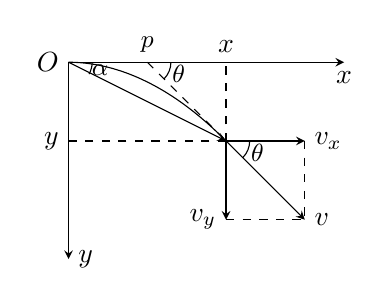
\begin{tikzpicture}
    \draw [->,>=stealth] (0,0) node [anchor= east] {$O$}--(3.5,0) node [anchor=north]{$x$};
    \draw [->,>=stealth] (0,0)--(0,-2.5) node [anchor=west]{$y$};
    \draw (0,0) parabola (2,-1);
    \draw [dashed] (1,0) node [anchor=south] {\small $p$} -- (2,-1);
    \draw (1.2121,-0.2121) arc (315:360:0.3);
    \draw (1.4,-0.15) node {\small $\theta$};
    \draw [dashed] (2,-1) --(2,0) node [anchor=south] {$x$};
    \draw [dashed] (2,-1) -- (0,-1) node [anchor=east] {$y$};
    \draw [->,>=stealth] (2,-1) -- (3,-2) node [anchor=west] {$v$};
    \draw [->,>=stealth] (2,-1) -- (3,-1) node [anchor=west] {$v_x$};
    \draw [->,>=stealth] (2,-1) -- (2,-2) node [anchor=east] {$v_y$};
    \draw [->,>=stealth] (0,0) -- (2,-1);
    \draw (0.2598,-0.15) arc (330:360:0.3);
    \draw (0.4,-0.1) node {\small $\alpha$};
    \draw [dashed] (3,-1) -- (3,-2);
    \draw [dashed] (2,-2) -- (3,-2);
    \draw (2.2122,-1.2122) arc (315:360:0.3);
    \draw (2.4,-1.15) node {\small $\theta$};
  \end{tikzpicture}
  \caption{平抛运动}
  \label{fig:parabolatwo}
\end{figure}

\subsection{平抛运动的速度}

水平方向做匀速直线运动,竖直方向做自由落体运动,则

\begin{gather}
  v_x=v_0 \\
  v_y=gt \\
  v=\sqrt{v_x^2+v_y^2}=\sqrt{v_0^2+g^2t^2} \\
  \tan\theta =\cfrac{v_y}{v_x}=\cfrac{gt}{v_0}
  \label{eq:ppv}
\end{gather}

\subsection{平抛运动的位移}

水平方向做匀速直线运动,竖直方向做自由落体运动,则

\begin{gather}
  x=v_0t\\
  y=\cfrac{1}{2}gt^2\\
  l=\sqrt{x^2+y^2}\\
  \tan \alpha =\cfrac{y}{x}=\cfrac{gt}{2v_0}
  \label{eq:ppl}
\end{gather}

\subsection{推论}

观察式 \eqref{eq:ppv}和式 \eqref{eq:ppl} 则可以得到,平抛运动速度与水平方向夹角的正切值是位移与水平方向正切值的二倍.即

\begin{equation}
  \tan\theta =2\tan \alpha
  \label{eq:ppthetaalpha}
\end{equation}

将速度方向径向延长,交$x$轴于点 p ,设p点与位移的横坐标相距为 $d$ ,则由式\eqref{eq:ppthetaalpha} 可得

\begin{gather}
  \tan\theta =2\tan \alpha \notag\\
  \cfrac{y}{d}=2\cfrac{y}{x} \notag\\
  d=\cfrac{x}{2}
  \label{eq:ppmiddle}
\end{gather}

由式\eqref{eq:ppmiddle}可知,速度反向延长线交 $x$轴于位移横坐标的中点.切线交于$x$坐标的中点,这是一个数学结论,所以不只是平抛运动适用,在所有的类平抛运动中都是成立的.

\section{圆周运动}
质点运动的轨迹是圆时称为圆周运动.当相同的时间质点经过的弧长相同时,质点的运动叫做匀速圆周运动.
\subsection{线速度}
线速度就是通常的速度,之所以这样称呼是为了区别与后文所定义的角速度.如下图

\begin{figure}[H]
  \centering
  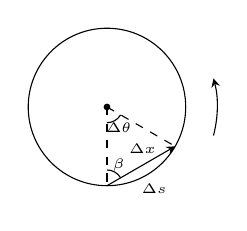
\begin{tikzpicture}
    \draw (0,0) circle [radius=1]; 
    \filldraw [black] (0,0) circle [radius=1pt];
    \draw [dashed] (0,0)--(0,-1);
    \draw [dashed] (0,0)--(330:1);
    \draw [->,>=stealth] (0,-1)--(330:1);
    \draw (270:0.2) arc (270:330:0.2);
    \draw (300:0.3) node {\tiny $\Delta\theta$};
    \draw (310:0.7) node {\tiny $\Delta x$};
    \draw (300:1.2) node {\tiny $\Delta s$};
    \draw[->,>=stealth] (345:1.4) arc (-15:15:1.4);
    \draw (0,-1)+(30:0.2) arc (30:90:0.2);
    \draw (0,-1)+(60:0.3) node {\tiny $\beta$};
  \end{tikzpicture}
  \caption{圆周运动}
  \label{fig:circle}
\end{figure}

由瞬时速度的定义得

\begin{equation}
  v=\lim_{\Delta t \to 0} \cfrac{\Delta x}{\Delta t}
  \label{eq:circv}
\end{equation}

由于
$$\lim_{\Delta t \to 0} \Delta x=\Delta s$$
所以式 \eqref{eq:circv} 又可以写作

\begin{equation}
  v=\lim_{\Delta t \to 0} \cfrac{\Delta s}{\Delta t}
  \label{eq:circvs}
\end{equation}

下面考察线速度的方向,由图 \ref{fig:circle} 可得
\begin{gather}
  2\beta +\Delta \theta =\pi \notag\\
  \beta =\cfrac{\pi}{2}-\cfrac{\Delta \theta}{2}
  \label{eq:vangle}
\end{gather}

由于当 $\Delta t \to 0$ 时, $\Delta \theta \to 0$ ,所以\eqref{eq:vangle}在此时为

\begin{equation}
  \beta =\cfrac{\pi}{2}
  \label{eq:vangletwo}
\end{equation}

由式 \eqref{eq:vangletwo} 可得:匀速圆周运动的速度与半径垂直.

\subsection{角速度}

描述圆周运动也可以使用质点绕圆心转过的角度,于是定义角速度为单位时间内质点绕圆心转过的弧度.即

\begin{equation}
  \omega = \lim_{\Delta t \to 0} \cfrac{\Delta \theta}{\Delta t}
  \label{eq:circomega}
\end{equation}

角速度也是一个矢量,它的方向由右手定则确定,即:右手四指与质点绕行的方向相同,则拇指所指示的方向就是角速度 $\omega$ 的方向.例如,当在纸平面内质点绕逆时针转动时,则 $\omega$ 的方向是垂直于纸面指向外,反之则顺时针时 $\omega $ 垂直于纸面指向里.

角速度的单位,由定义式 \eqref{eq:circomega} 可得为 $ s^{-1}$ ,这是因为弧度是无量纲数,但是历史上为了称呼的方便,仍然配合数学上弧度的定义,叫角速度的单位为 $rad/s$.

\subsection{线速度与角速度的关系}

数学上关于弧度的定义为弧长比上半径,即

\begin{equation*}
  \Delta \theta =\cfrac{\Delta s}{r}
\end{equation*}

上式中的弧度 $\Delta \theta$ 和 弧长 $\Delta s$ 都上质点在 $\Delta t$ 内所发生的,所以在上式中左右同时除以 $\Delta t$ ,再由角速度和线速度的定义式\eqref{eq:circomega} 和 \eqref{eq:circvs}便得到

\begin{gather}
  \cfrac{\Delta \theta}{\Delta t}=\cfrac{\frac{\Delta s}{\Delta t}}{r} \notag \\
  \omega =\cfrac{v}{r}
  \label{eq:circleomegav}
\end{gather}

式 \eqref{eq:circleomegav} 又可以写为 $v=\omega r$.

\subsection{周期}

质点绕圆心转一周所用的时间称为周期,用大写字母 $T$ 表示.

\subsection{角速度与周期的关系}

据角速度的定义式 \eqref{eq:circomega} 可得,当质点绕圆周一周时所转过的弧度为 $2\pi$,其所需时间为一个周期 $T$ ,所以角速度与周期的关系为

\begin{equation}
  \omega =\cfrac{2\pi}{T}
  \label{eq:omegaT}
\end{equation}

\subsection{转速}

转速的定义为单位时间内质点绕圆心转过的圈数.用字母 $n$ 表示.由于转一圈用时 $T$ ,所以单位时间内转过的圈数为

\begin{equation}
  n=\cfrac{1}{T}
  \label{eq:circnT}
\end{equation}

由角速度与周期的关系 \eqref{eq:omegaT} 和式 \eqref{eq:circnT} 对比可得

\begin{equation}
  \omega =2\pi n
  \label{eq:onegan}
\end{equation}

\subsection{转速与频率的区别}

转速的定义为 $n=\frac{1}{T}$ 频率的定义也是 $f=\frac{1}{T}$ ,从定义上来看这二者是相同的.但是它们的单位通常又不相同,转速的单位是 $ r/min$ ,频率的单位是 $H_z$ ,然而这两个单位转换以后是相同的.所以它们的单位可以认为是相同的.

转速和频率的根本区别在于它们的描述能力!所有的周期性运动都可以用频率描述,比如一个在直线上做往复运动的小球,钟摆的周期性摆动等都可以用频率来描述,但是它们不是圆周运动,而转速只能用来描述圆周运动.

\section{向心加速度}

这一节我们来推导匀速圆周运动的加速度 $a$,在后面的论述中我们可以得到它的方向始终指向质点所做圆周运动的轨迹的圆心,所以称呼它为 向心加速度.
\begin{figure}[H]
  \centering
  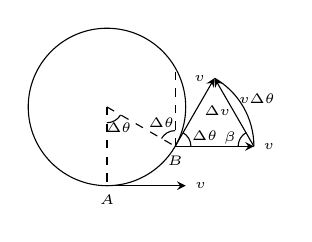
\begin{tikzpicture}
    \draw (0,0) circle [radius=1]; 
    \draw [dashed] (0,0) --(270:1);
    \draw [->,>=stealth](0,-1)--(1,-1) node [anchor=west] {\tiny $v$};
    \draw [dashed] (0,0) --(330:1);
    \draw [->,>=stealth] (330:1) -- +(60:1) node [anchor=east] {\tiny $v$};
    \draw [->,>=stealth] (330:1) -- +(1,0) node [anchor=west] {\tiny $v$};
    \draw [->,>=stealth] (330:1)+(1,0)--+(60:1);
    \draw (270:0.2) arc (270:330:0.2);
    \draw (300:0.3) node {\tiny $\Delta\theta$};
    \draw (330:1)+(0.2,0) arc (0:60:0.2);
    \draw (330:1)+(20:0.4) node {\tiny $\Delta\theta$};
    \draw (330:1)+(1,0) arc (0:60:1); 
    \draw (1.866,-0.5)+(120:0.2) arc (120:180:0.2);
    \draw (1.866,-0.5)+(135:0.15) node [anchor=east] {\tiny $\beta$};
    \draw (330:1)+(40:0.7) node {\tiny $\Delta v$};
    \draw (330:1)+(30:1.2) node {\tiny $v\Delta \theta$};
    \draw (270:1) node [anchor=north]{\tiny $A$};
    \draw (330:1) node [anchor=north] {\tiny $B$};
    \draw [dashed] (330:1)--+(90:1);
    \draw (330:1)+(90:0.2) arc (90:150:0.2);
    \draw (330:1)+(120:0.35) node {\tiny $\Delta \theta$};
  \end{tikzpicture}
  \caption{向心加速度}
  \label{fig:circleaccelerate}
\end{figure}

图 \ref{fig:circleaccelerate} 所描述的是经过时间 $\Delta t$ 后质点由$A$ 点运动到 $B$点,将$A$的瞬时速度平移到点 $B$ ,并以$B$ 点为圆心,$v$ 的长度为半径作弧.则速度所发生的角度变化与半径所发生的角度变化相同,都是 $\Delta \theta$.当 $\Delta t \to 0$ 时有
 
\begin{equation*}
  \Delta v =v\Delta\theta
\end{equation*}

由加速度的定义式 \eqref{eq:instantaneous acceleration} 可以得到质点做匀速圆周运动时的加速度为
\begin{gather}
  a=\cfrac{\Delta v}{\Delta t} \notag \\
  a=\cfrac{v\Delta\theta}{\Delta t} \notag\\
  a=v\omega
  \label{eq:xiangxina}
\end{gather}

将式 \eqref{eq:circleomegav} 代入式 \eqref{eq:xiangxina}得

\begin{equation}
  a=\cfrac{v^2}{r}
  \label{eq:xiangxinav}
\end{equation}

由式\eqref{eq:circleomegav} 解得 $v=\omega r$ 代入式 \eqref{eq:xiangxina}得

\begin{equation}
  a=\omega^2r
  \label{eq:xiangxinaomega}
\end{equation}

将式 \eqref{eq:omegaT} 代入式 \eqref{eq:xiangxinaomega} 得

\begin{equation}
  a=\cfrac{4\pi^2}{T^2}r
  \label{eq:xiangxinaT}
\end{equation}

\section{Kepler 行星运动定律}

这一节介绍行星绍太阳运动的规律,使用这三大规律可以解决若干与行星运动有关的题目,最大的应用应该就是结合 Newton 的三大定律来推导出万有引力定律.

\subsection{Kepler 第一定律(椭圆轨道定律)}

行星绕太阳运行的轨道是一个椭圆,太阳处于椭圆轨道的一个焦点上.

\begin{figure}[H]
  \centering
  \begin{tikzpicture}
    \draw (0,0) ellipse (1 and 0.8);
    \draw (-0.6,0) circle [radius=5pt];
    \draw (-0.5,0) node [anchor=west] {\tiny \mbox{太阳}};
    \filldraw (0,0.8) node [anchor=south] {\tiny \mbox{行星}} circle [radius=2pt];
  \end{tikzpicture}
  \caption{Kepler 第一定律}
  \label{fig:kepler1}
\end{figure}

\subsection{Kepler 第二定律(等面积定律)}

同一颗行星在轨道的不同位置,在相同的时间内行星与太阳中心的连线扫过的面积相等,即图\ref{fig:kepler2}所示的相同的时间内,行星与太阳连线所扫过的任意二个阴影面积相等.

\begin{figure}[H]
  \centering
  \begin{tikzpicture}
    \draw (0,0) ellipse (1 and 0.8);
    \draw (-0.6,0) circle [radius=5pt];
    \draw (-0.5,0) node [anchor=west] {\tiny \mbox{太阳}};
    \filldraw (0,0.8) node [anchor=south] {\tiny \mbox{行星}} circle [radius=2pt];
    \draw[pattern=north west lines] (-0.6,0) -- (0,0.8) arc (90:60:1 and 0.8)--(-0.6,0); 
    \draw[pattern=north west lines] (-0.6,0) -- (-0.5,-0.692820323) arc (240:280:1 and 0.8)--(-0.6,0); 
    \draw (-1,0) node [anchor=east] {\tiny $A$}--(1,0) node [anchor=west]{\tiny $B$};
    \draw [->,>=stealth] (-1,0)--(-1,-0.7) node [anchor=east] {\tiny $v_A$};
    \draw [->,>=stealth] (1,0)--(1,0.5) node [anchor=west] {\tiny $v_B$};
    \draw (-0.8,0) node  {\tiny $r_A$};
    \draw (0.5,0) node {\tiny $r_B$};
  \end{tikzpicture}
  \caption{Kepler 第二定律}
  \label{fig:kepler2}
\end{figure}

行星在近日点和远日点与左焦点的距离分别为$r_A$ 和 $r_B$ ,由Kepler 第二定律可以得到行星在这二点的一个特例情况

\begin{equation}
  v_Ar_A=v_Br_B
  \label{eq:kepler22}
\end{equation}

\subsection{Kepler 第三定律(周期定律)}

不同行星绕太阳运行时,它们的半长轴的三次方与周期的平方的比值是一个常数.即

\begin{equation}
  \cfrac{a^3}{T^2}=k \qquad (\mbox{k为Kepler 常数})
  \label{eq:kepler3}
\end{equation}

\begin{figure}[H]
  \centering
  \begin{tikzpicture}
    \draw (0,0) ellipse (1 and 0.8);
    \draw (-0.6,0) circle [radius=5pt];
    \draw (-0.5,0) node [anchor=west] {\tiny \mbox{太阳}};
    \filldraw (0,0.8) node [anchor=south] {\tiny \mbox{行星1}} circle [radius=2pt];
    \draw (0,0) ellipse (1.4 and 1.2649);
    \filldraw (1.4,0) node [anchor=west] {\tiny \mbox{行星2}} circle [radius=4pt];
  \end{tikzpicture}
  \caption{Kepler 第三定律}
  \label{fig:kepler3}
\end{figure}

如图 \ref{fig:kepler3} 所示,则此时Kepler 第三定律可以表达为

\begin{equation}
  \cfrac{a_1^3}{T_1^2}=\cfrac{a_2^3}{T_2^2}
  \label{eq:kepler33}
\end{equation}

\section{万有引力定律}

这一节我们利用Kepler 三大定律推导万有引力定律,但是在高中阶段大家还不能处理极坐标系下椭圆的计算,所以我们必须对Kepler三大定律做一定的简化工作.

\subsection{Kepler 第一定律的简化}

地球绕太阳运行的轨道近似为圆,圆也是一种特殊的椭圆,它的离心率为零.

\subsection{kepler 第二定律的简化}

由Kepler 第三定律得,相同时间内行星与太阳中心的连线所扫过的面积相等,可以得出当轨道为圆时,半径不变,则任何相同的时间内半径所扫过的弧长相等,也就是行星绕太阳的运动可以近似为:匀速圆周运动.这样就可以使用匀速圆周运动的规律来推导万有引力定律.

\subsection{Kepler 第三定律的简化}

由于轨道为圆时,半径就是半长轴,所以Kepler 第三定律简化为

\begin{equation}
  \cfrac{r^3}{T^2}=k
  \label{eq:kepler3jianhua}
\end{equation}

\subsection{推导万有引力定律}
 
首先,我们选择太阳为参考系,则行星绕太阳做匀速圆周运动,太阳对行星的引力提供了行星绕太阳运动的向心力.记太阳的质量为 $M$ ,行星的质量为 $m$ ,行星绕太阳运动的周期为 $T$,行星与太阳的距离为$r$ ,则由 Newton 第二定律得太阳对行星的引力 $F$ 为

\begin{gather}
  F=m\cfrac{4\pi^2}{T^2}r \notag\\
  F=m4\pi^2 \cdot \cfrac{r^3}{T^2} \cdot \cfrac{1}{r^2} 
  \label{eq:kn2}
\end{gather}

将 Kepler 第二定律 \eqref{eq:kepler3jianhua} 代入式 \eqref{eq:kn2}得太阳对行星的引力为

\begin{equation}
  F=\cfrac{4\pi^2km}{r^2}
  \label{eq:kn21}
\end{equation}

同理,我们也可以选择行星为参考系,则太阳绕行星做匀速圆周运动,它们的距离仍然是 $r$ ,但是太阳绕行星的周期却与行星绕太阳的周期不同(比如地球绕太阳一周是一年,但是太阳绕地球一周却是一天),这就导致了 Kepler 常数的不同.此时可以计算行星对太阳的引力 $F'$  为

\begin{gather}
  F'=M\cfrac{4\pi^2}{T'^2}r \notag \\
  F'=M4\pi^2 \cdot \cfrac{r^3}{T'^2} \cdot \cfrac{1}{r^2}
  \label{eq:kn22}
\end{gather}

将Kepler 第三定律 \eqref{eq:kepler3jianhua} 代入式 \eqref{eq:kn22}得


\begin{equation}
  F'=\cfrac{4\pi^2k'M}{r^2}
  \label{eq:kn23}
\end{equation}

由 Newton 第三定律得 $F'=F$ 也就是

\begin{equation*}
  \cfrac{4\pi^2k'M}{r^2}=\cfrac{4\pi^2km}{r^2}
\end{equation*}

由上式得

\begin{equation}
  \cfrac{4\pi^2k}{4\pi^2k'}=\cfrac{M}{m}
  \label{eq:kn24}
\end{equation}

式 \eqref{eq:kn24} 只是一个比例相等,不能得出分子对应相等和分母对应相等.例如

\begin{equation*}
  \cfrac{9}{6}=\cfrac{3}{2}
\end{equation*}

在上式中,右式中如果分子分母同时乘以$3$则可以得出分子对应相等,即 $9=3\times 3$ ;分母也对应相等,即 $6=2\times 3$ .所以在式 \eqref{eq:kn24} 中,只要在右式中分子分母同时乘上一个常数 $G$ ,也可以得到左式和右式中分子分母对应相等,这里 $G$仅仅是一个数学上的常数,其数值应当由实验测定.即


\begin{equation}
  \cfrac{4\pi^2k}{4\pi^2k'}=\cfrac{GM}{Gm}
  \label{eq:kn25}
\end{equation}

由上式得

\begin{gather}
  4\pi^2k=GM \label{eq:kconst1}\\
  k=\cfrac{GM}{4\pi^2}
  \label{eq:kconst2}
\end{gather}

将式 \eqref{eq:kconst1} 代入太阳对行星的引力式 \eqref{eq:kn21} 中,得太阳对行星的引力

\begin{equation}
  F=G\cfrac{Mm}{r^2}
  \label{eq:wyyl1}
\end{equation}

Newton 认为不仅太阳对行星的引力具备上述表达形式,世界上任何可视为质点的两个物体间都应当具备上述形式的引力,设任意二个可视为质点的两个物体的质量分别为 $m_1$ 和 $m_2$ ,则有

\begin{equation}
  F=G\cfrac{m_1m_2}{r^2}
  \label{eq:wyyl2}
\end{equation}

式\eqref{eq:wyyl2} 就是万有引力公式.公式中的常数是作为一个数学要求引入的,所以它与任何物体都没有关系,称为万有引力常量.当采用国际单位时,它的数值是

\begin{equation}
  G=6.67\times 10^{-11} N\cdot m^2/kg^2
  \label{eq:wyylG}
\end{equation}

万有引力常量的数值由美国物理学家 Cavendish 使用扭称实验测定.

\section{万有引力的严格求解}

这一节的目的在于使用椭圆规律来严格求解万有引力定律,也是为了说明在圆轨道中的一些规律在也符合椭圆的一般情况.

\subsection{比耐公式}

\begin{gather*}
  \overset{.}{\overrightarrow{r}}= \overset{.}{r} \vec{i}+r\overset{.}{\theta}\vec{j} \\
  \overset{..}{\overrightarrow{r}}=(\overset{..}{r}-r\overset{.}{\theta}^2)\vec{i}+(2\overset{.}{r}\overset{.}{\theta}+r\overset{..}{\theta})\vec{j}\\
  \overset{..}{\overrightarrow{r}}=(\overset{..}{r}-r\overset{.}{\theta}^2)\vec{i}+\frac{1}{r}\frac{d}{dt}(r^2\overset{.}{\theta})\vec{j}
\end{gather*}

由 Kepler 第二定律可知,$r^2\overset{.}{\theta}=\mbox{常数}$,记此常数为 $h$于是位矢对时间的二次微分,即加速度只有径向分量

\begin{gather}
  \overset{..}{\overrightarrow{r}}=(\overset{..}{r}-r\overset{.}{\theta}^2)\vec{i}
  \label{eq:rdd}\\
  \dot r =\frac{dr}{d\theta}\dot \theta =\frac{h}{r^2}\frac{dr}{d\theta}=-h\frac{du}{d\theta} \qquad (u=\frac{1}{r})\\
  \ddot r =-h\dot \theta \frac{d^2u}{d\theta^2}=-h^2u^2\frac{d^2u}{d\theta^2} 
\end{gather}

同时 $r{\dot \theta}^2=h^2u^3$ 所以Newton 第二定律表达为

\begin{equation}
  -h^2u^2(\frac{d^2u}{d\theta^2}+u)=\frac{F}{m}
  \label{eq:binai}
\end{equation}

式 \eqref{eq:binai} 就是有心力场中的比耐公式.

\subsection{椭圆参数关系}

椭圆的标准方程为

\begin{equation}
  r=\frac{P}{1-e\cos\theta}
  \label{eq:tuoyuan}
\end{equation}

由式 \eqref{eq:tuoyuan} 可得

\[ \left.
\begin{gathered}
  a+c=\frac{P}{1-e}  \\
  a-c=\frac{p}{1+e} 
\end{gathered}
\right\}
\implies 
  a^2-c^2=\frac{p^2}{1-e^2} 
\implies 
  b^2=ap
\]

\subsection{万有引力的严格推导}

由Kepler 第一定律得:

\begin{equation}
  r=\frac{p}{1-e\cos\theta}
  \implies
  u=\frac{1}{r}=\frac{1-e\cos\theta}{p}
  \label{eq:kepleru}
\end{equation}

选择太阳为参考系,计算太阳对行星的引力,将式 \eqref{eq:kepleru} 代入式 \eqref{eq:binai} 可得此引力 $F$ 为

\begin{equation}
  F=-h^2mu^2\cdot\frac{1}{p}
  \label{eq:newkn}
\end{equation}

由 Kepler 第二定律可得 :
\begin{equation}
   h=r^2\dot \theta =\frac{2\pi ab}{T}
  \label{eq:newkn1}
\end{equation}

将式 \eqref{eq:newkn1} 代入式 \eqref{eq:newkn} 得

\begin{equation}
  F=-\frac{4\pi^2ma^2b^2}{pT^2}\cdot \frac{1}{r^2}
  \label{eq:newkn2}
\end{equation}

由椭圆关系 $b^2=ap$ 代入式 \eqref{eq:newkn2}得

\begin{equation}
  F=-4\pi^2m\frac{a^3}{T^2}\cdot \frac{1}{r^2}
  \label{eq:newkn3}
\end{equation}

将Kepler 第三定律 \eqref{eq:kepler3}代入式 \eqref{eq:newkn3} 得

\begin{equation}
  F=-\frac{4\pi^2km}{r^2}
  \label{eq:newwyyl}
\end{equation}

同理可以得出行星对太阳的引力

\begin{equation}
  F'=-\frac{4\pi^2k'M}{r^2}
  \label{eq:newwyyl1}
\end{equation}

由 Newton 第三定律得$F'=F$ 则

\begin{equation}
  \cfrac{4\pi^2k}{4\pi^2k'}=\cfrac{GM}{Gm}
  \label{eq:newwyyl2}
\end{equation}

由上式\eqref{eq:newwyyl2}得

\begin{gather}
  4\pi^2k=GM \label{eq:newkconst1}\\
  k=\cfrac{GM}{4\pi^2}
  \label{eq:newkconst}
\end{gather}

将式 \eqref{eq:newkconst1} 代入太阳对行星的引力式 \eqref{eq:newwyyl} 中,得太阳对行星的引力

\begin{equation}
  F=-G\cfrac{Mm}{r^2}
  \label{eq:newwyyl3}
\end{equation}

Newton 将上式推广到任意二个质点间都存在上述形式的引力,称为万有引力.即

\begin{equation}
  F=-G\cfrac{m_1m_2}{r^2}
  \label{eq:newwyyl4}
\end{equation}
